\newpage\null\thispagestyle{empty}\newpage
\clearpage{\thispagestyle{empty}\cleardoublepage}
\part{Basics}
% \cleanchapterquote{We are part of the universe that has developed a remarkable ability: We can hold an image of the world in our minds. We are matter contemplating itself.}{Sean Carroll}{The Particle at the End of the Universe}
% \acbarrier
\parttoc
% 
% 
% 
\cleardoublepage
\setcounter{chapter}{1}
\chapter{Neuroanatomy}
\label{chap:neuro}
%
% \paragraph{TODO}
% \begin{itemize}
%     \item was für parameter treten wo im Gehirn auf
% \end{itemize}
%
%
\section{Introduction}
%
Neuroanatomy is the study of the structure of the brain.
Its describing regions and the structure of the nervous system in humans and animals.
Techniques such as \ac{dMRI}, fluorescence microscopy, microscopy on stained tissue, autoradiography (to name a few), have been able to study more and more structures from different perspectives in the brain with different resolutions, modalities and contrasts on different species.
% 
\par
%
This chapter gives a general overview of the structure of the brain with its most important regions as well as the nerve fiber architecture.
More in-depth information can be found, for example, in the following literatures \dummy{}.
% 
%
% 
% The human brain is one of the most complex organs with a great diversity of cells, connections, topography and resulting functionalities.
% 
% 
%
\section{Brain Architecture}
%
The mammal brain consists of three main parts: the brainstem, the cerebellum and the cerebrum (see \cref{fig:humanBrain}).
% 
The brainstem is the connection between the different brain areas and the spinal cord located at the bottom of the brain.
It can be further subdivided into the midbrain, the pons and the medulla obiongata.
The cerebellum is located at the lower rear of the brain. Its most important function is motor control.
It is highly folded \todo{species?} and therefore has a particularly large surface area.
The cerebrum is the largest part of the human brain.
As the cerebellum its surface is folded as well \todo{species?}.
The cerebrum is split into a left and right hemisphere.
In addition, the cerebrum can be divided into four parts:
the frontal, parietal, temporal, and occipital lobes (see \cref{fig:brainLobes}).
The frontal lobe is responsible for voluntary movements of specific body parts as well as the human personality.
The parietal lobe's main functionalities are the processsing of the sensory informations.
The primary function of the occipital lobe is signal processing of the visual system.
The temporal lobe contains auditory functions and language perception in addition to visual memories.
Beneath the brain surface there are also other structures such as the basal gangila or the thalamus.
\par
% 
\begin{figure}[!t]
\centering
\subcaptionbox{%
        \label{fig:brainLobes}%
        Sagital view of the human brain with lobes colored in: {\color[RGB]{117,112,179}frontal}, {\color[RGB]{230,171,2}parietal}, {\color[RGB]{27,158,119}temporal} and {\color[RGB]{231,41,138}occipital} lobe.
        The {\color[RGB]{102,166,30}cerebellum} is at the bottom, with the {\color[RGB]{217,95,2}brainstem} next to it.
        Modivied version of \url{https://en.wikipedia.org/wiki/Frontal_lobe}%
    }[.47\textwidth]{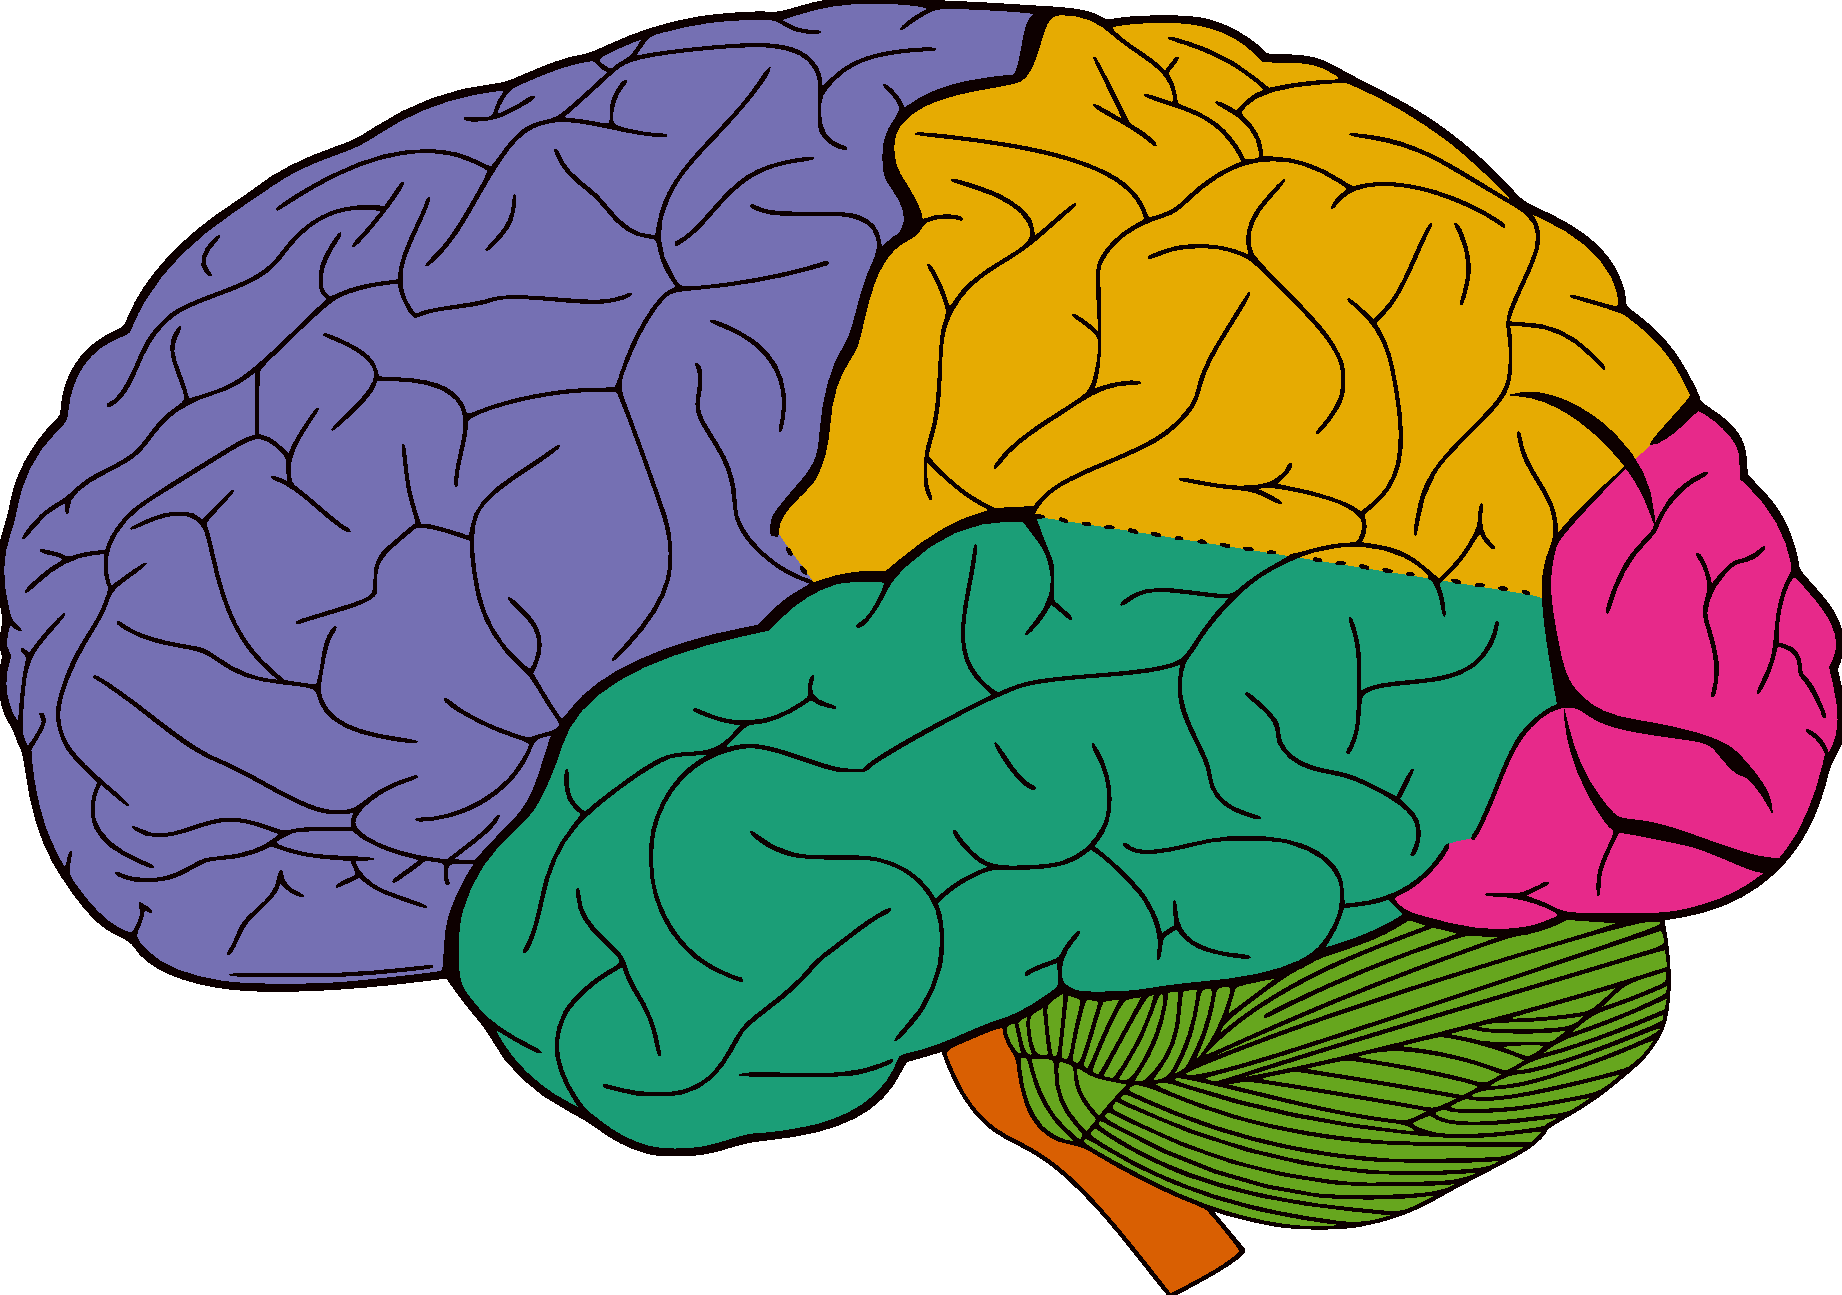
\includegraphics[height=0.3\textwidth]{gfx/neuroanatomy/brain_lobes.pdf}}
\hfill
\tikzset{external/export next=false}
\subcaptionbox{%
        \label{fig:coronalStained}%
        \todo{BB 4201} Coronal section stained for cell bodies. The \ac{GM} is dark while the \ac{WM} is bright. The left and right hemisphere is connected via the corpus calosum.}%
    [0.47\textwidth]{\includegraphics[height=0.3\textwidth]{dev/brain/BB_4201.png}}
    % \begin{tikzpicture}[]
    %     \node[inner sep=0pt, anchor = south west] (fig) at (0,0)
    %     {\includegraphics[height=0.3\textwidth]{dev/brain/BB_4201.png}};
    %     \coordinate (WM1) at ($(fig.north west)!0.6!(fig.north east)$);
    %     \coordinate (WM2) at ($(fig.north east)!0.35!(fig.south east)$);
    %     \draw[RED, ultra thick, <-] (WM1 |- WM2) -- ++ (-42:0.75) node[pos=1, anchor=north] {\textbf{WM}};
    %     \coordinate (GM1) at ($(fig.north west)!0.275!(fig.north east)$);
    %     \coordinate (GM2) at ($(fig.north east)!0.125!(fig.south east)$);
    %     \draw[GREEN, ultra thick, <-] (GM1 |- GM2) -- ++ (-65:0.75) node[pos=1, anchor=north] {\textbf{GM}};
    % \end{tikzpicture}
% }
\caption{Illustration of the human brain and a cell body stained coronal section.}
\label{fig:humanBrain}
\end{figure}
%
The cerebellum and cerebrum contain a \ac{GM} stucture at the brain surface.
This structure is filled with neurons.
These cells have the task of processing the information of all signals coming from inside and outside of the brain.
These cells are arranged in cortical layers that have different thicknesses, cell types, and densities specific to a brain area.
These cells have a relatively high density and are not only locally interconnected with each other, but connect also with different brain areas.
%  (see \cref{fig:nerveFiber,fig:cortLayers}).
Therefore, the folding of the brain is particularly important to increase the surface and therefore the number of cells.
In the human brain there are several billions of nerve cells.
There are many types of cells, \eg{} granule or pyramidal cells.
The highly interconnected structure and arrangement of the various cells is the source of its high number of different functionalities.
It is imporatant to investiagte the human brain to gain a better understanding of the brain's function and an improved understanding of pathophysiological processes that may lead to improved medical treatment of brain deseases.
%
%
%
\section{Fiber architecture} \label{sec:fiberArchitecture}
%
\begin{figure}[!t]
\centering
% \subcaptionbox{
%     \label{fig:cortLayers}
%     Cortical layers \todo{wichtig?}
%     }[0.225\textwidth]{\includegraphics[height=4.5cm]{dev/wiki/layers.png}}
% \hfill
\tikzset{external/export next=false}
% \subcaptionbox{
%     \label{fig:nerveCell}
%     Nerve cell structure.
% }[0.75\textwidth]{
\begin{tikzpicture}[every node/.style={font=\small,},]
    \node[inner sep=0pt, anchor = south west] (fig) at (0,0) {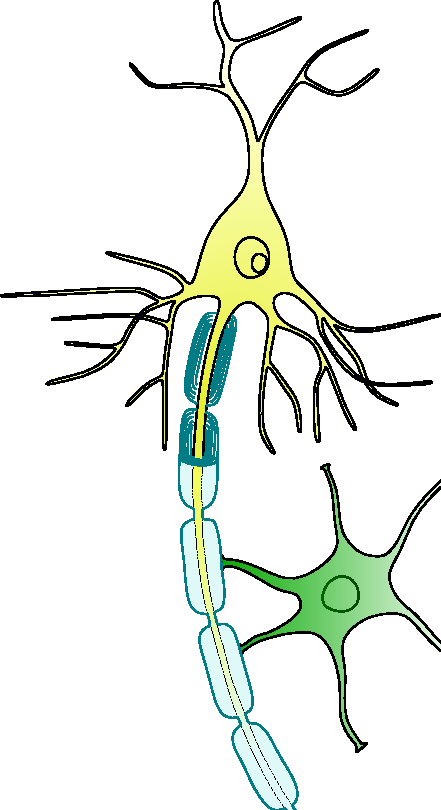
\includegraphics[ angle=90,width=0.75\textwidth]{gfx/neuroanatomy/neuron-axon.pdf}}; %height=4.2cm
    \begin{scope}[overlay]
        % \foreach \p in {0,0.1,0.2,0.3,0.4}{
        %     \draw[blue] (rel cs:name=fig,x=\p,y=\p) rectangle (rel cs:name=fig,x=1-\p,y=1-\p);
        % }
        % 
        \node[anchor=south] at (rel cs:name=fig,x=0.72,y=1.025) {Oligodendrocyte};
        \node[anchor=north] at (rel cs:name=fig,x=0.235,y=0.22) {Cell Body};
        \node[anchor=west] at (rel cs:name=fig,x=1,y=0.675) {Axon};
        \node[anchor=north] at (rel cs:name=fig,x=0.7,y=0.4) {Myelin};
        \draw[<-] (rel cs:name=fig,x=0.9,y=0.5) -- ++(-69:0.5) node[pos=1,anchor=north] {Node of Ranvier};
        \draw[<-] (rel cs:name=fig,x=0.295,y=0.53) -- ++(-140:0.75) node[pos=1,anchor=north] {Nucleus};
        \node[anchor=south] at (rel cs:name=fig,x=0.24,y=0.8) (D) {Dendrites};
        \draw[->] (rel cs:name={D},x=0.3,y=0) -- ++(-155:0.6){};
        \draw[->] (rel cs:name={D},x=0.7,y=0) -- ++(-25:0.6){};
    \end{scope}
    \path[] ($(fig.south west)-(0,0)$) rectangle ($(fig.north east)+(1,0.75)$);
\end{tikzpicture}
% }
\caption{Illustration of a neuron with axon and oligodendrocytes. The olegodendrocyte build up a layered lipid structure up, surrounding the axon. The myelin layers are separated along the axon by nodes of Ranvier.}
\label{fig:CortexAndNerveCell}
\end{figure}
%
Nerve cells are connected by nerve fibers.
A typical nerve cell (see \cref{fig:nerveCell}) comprises a cell body, called a soma, that processes incoming information.
The information arrives via dendrites, which are star-shaped branches.
The axon is the cell's only information output.
It travels through the brain often associated with nerve fiber bundles to its destination, where it connects with the axon terminal to other neurons.
\par
%
The axon is surrounded by a myelin sheath, a lipid layered structure deriving from nearby olegodendrides (see \cref{fig:human-brain}).
The myeling electrically insulates the axon and improves the speed of propagation of the electrical action potential along the axon and also its signal strength.
The diamater of the myelin ranges from about $\SI{0.5}{\micro\meter}$ to several $\si{\micro\meter}$ (see \cref{tag:axonDiameter}).
There are many different types of axons.
Some contain a very thick myelin layer, while others have none.
The high density of axons and myelin makes the brainappear white and is therefore called \ac{WM}, whereas the outer cell bodys appear darker and ist called \ac{GM}.
This color difference is clearly visible in a Nissle stained histological sections (see \cref{fig:coronalStained}).
\par
%
To enhance the contrast of the nerve fibers to the background, staining like Nissle is used to darken the myelin (see \cref{fig:brainMyelinStain}).
This allows to follow small nerve fibers down to individual nerves depending on their myelination degree.
Larger nerve fiber bundles are such dark, that mostly no orientation can be exracted.
\par
% 
\Cref{fig:brainMyelinStain} shows a nissle stained example. 
\todo{...}.
\par
% 
\begin{figure}[!t]
	\centering
	\tikzset{external/export next=false}
	\begin{tikzpicture}[]  
        \node[inner sep=0pt, anchor = south west] (fig) at (0,0)
           {\includegraphics[width=\textwidth]{gfx/neuroanatomy/NeuralNet-BrainAtlasDotOrg.png}};
        %  
        \coordinate (A) at (fig.west);
        \coordinate (B) at (fig.west);
        %  
        \draw[Orange, ultra thick] (7.65,6.15) ellipse (1 and 0.5);
        \draw[ProcessBlue, ultra thick] (10,4.5) ellipse (2 and 1);
        % \draw[yellow, ultra thick] (fig.north west) -- ++ (13.87303cm,0);
    \end{tikzpicture}
	\caption[Myelin staining of the human thalamus]{Myelin staining of the human thalamus, sagital section. \textcolor{Orange}{Nerve fiber bundle} structures are visiable as \dummy{}. In between \textcolor{ProcessBlue}{net-like structures} are fromed from individual nerve fibers. \url{http://brainmaps.org/HBP3/h.sapiens/sag/h5thal-myelin/17a}}
	\label{fig:brainMyelinStain}
\end{figure}
% 
A nerve fiber bundle is a very complex structure, usually formed by multiple nerve fibers which form a bundle.
\Cref{fig:elecMic} shows an electron microscop image with segmentation of individual axons.
% 
\begin{figure}[!t]
	\centering
	\subcaptionbox{}[.49\textwidth]{
	    \includegraphics[width=0.45\textwidth]{dev/brain/auto_seg_axon_0.png}}\hfill
    \subcaptionbox{}[.49\textwidth]{
        \includegraphics[width=0.45\textwidth]{dev/brain/auto_seg_axon_1.png}}
	\caption{Automatic segmentet nerve fiber tissue from an electron microscope \cite{Abdollahzadeh2019}.}
	\label{fig:elecMic}
\end{figure}
% 
%
%
\section{Axon Literature}
\label{sec:axonMicroscopy}
%
\Cref{tab:axonDiameter} lists the results of the nerve fiber diameter. In summary the diameter is in the range of .
\par
% 
From studies with \ac{dMRI} and electron microscopy
\cite{Stikov2015,Dean2016,Mohammadi2015,Cercignani2017,Berman2018,Jung2018} the $g_{\mathit{ratio}}$ is in the range of $\SI{0.6}{}$ to $\SI{0.9}{}$, depending on the region (see \cref{tab:gratio}).
The $g_{\mathit{ratio}}$ describes the fraction of the axon to the entire nerve fiber diameter.
%
\begin{table}[!b]
\centering
\pgfplotstabletypeset[
    thesisTableStyle,
    font=\footnotesize,
    % col sep=comma,
    columns/area/.style={string type},
    columns/mean/.style={string type},
    columns/std/.style={string type},
]{
    area mean std
    {sup. longitudinal fascide} $\SI{0.8}{\micro\meter}$ $\SI{0.2}{\micro\meter}$
    {Unicate/inferior occipital fasc.} $\SI{0.51}{\micro\meter}$ $\SI{0.05}{\micro\meter}$
    {corpus calosum} $\SI{0.69}{\micro\meter}$ $\SI{0.04}{\micro\meter}$
}
\caption{Nerve fiber diameter distribution of the human brain. Mean values over three human brains \cite{Liewald2014}.}
\label{tab:axonDiameter}
\end{table}
%
\begin{table}[!b]
\centering
\pgfplotstabletypeset[
thesisTableStyle,
font=\footnotesize,
col sep=semicolon,
columns={article,cite,gratio},
columns/article/.style={string type, column name=study, column type = {l}},
columns/cite/.style={string type, column name=cite, column type = {l}},
columns/gratio/.style={string type, column name=$g_{\mathit{ratio}}$},
]{data/gratio.csv}
\caption{human $g_{\mathit{ratio}}$ from invivo mri studies.}
\label{tab:gratio}
\end{table}